
\chapter{Pruebas unitarias}

\section{Implementación de pruebas unitarias}
\subsection{Herramienta utilizada}
La herramienta que se utilizó para realizar las pruebas es \texttt{Vitest}.

\subsection{Implementación de test}

Se implementaron nueve pruebas unitarias utilizando \textbf{Vitest}, con el objetivo de verificar el comportamiento de las principales funciones de cálculo y procesamiento de fechas relacionadas con las fases lunares. Las pruebas se encuentran organizadas en el archivo \texttt{tests/ta.test.ts} y evalúan funciones del módulo \texttt{frontend/src/core/ta.ts}.

Las pruebas implementadas son las siguientes:

\begin{enumerate}
    \item \textbf{Validación de una fecha válida:} se verifica que la función \texttt{validateDate()} acepte correctamente una fecha válida sin generar una excepción.

    \item \textbf{Validación de una fecha inválida:} se comprueba que \texttt{validateDate()} genere una excepción cuando recibe un valor de fecha no válido.

    \item \textbf{Cálculo del día juliano:} se verifica que la función \texttt{julianDay()} obtenga correctamente el día juliano para una fecha de referencia. Para el caso utilizado en la prueba, el resultado esperado es aproximadamente \(2451545.0\).

    \item \textbf{Cálculo de la fase lunar:} se comprueba que \texttt{moonPhase()} devuelva un valor dentro del intervalo válido de \(0\) a \(1\), correspondiente a la representación de la fase lunar.

    \item \textbf{Identificación de Luna nueva:} se verifica que \texttt{phaseName()} identifique correctamente el valor de fase \(0\) como ``Luna nueva''.

    \item \textbf{Identificación de Luna llena:} se comprueba que \texttt{phaseName()} identifique correctamente el valor de fase \(0.5\) como ``Luna llena''.

    \item \textbf{Cálculo de iluminación:} se verifica que \texttt{illumination()} obtenga aproximadamente un \(100\% \) de iluminación para una fase de \(0\).

    \item \textbf{Diferencia entre fechas:} se comprueba que \texttt{daysBetween()} calcule correctamente la cantidad de días entre dos fechas. Para las fechas utilizadas en la prueba, el resultado esperado es de 9 días.

    \item \textbf{Formato de tiempo relativo:} se verifica que \texttt{formatRelativeTime()} devuelva ``Hoy'' cuando recibe un valor de cero días.
\end{enumerate}

La ejecución de estas pruebas se realiza desde la raíz del proyecto mediante el comando:

\begin{lstlisting}
npm test
\end{lstlisting}


\newpage
\subsection{Evidencia de ejecución de los tests}

Pruebas unitarias
\begin{figure}[H]
    \centering
    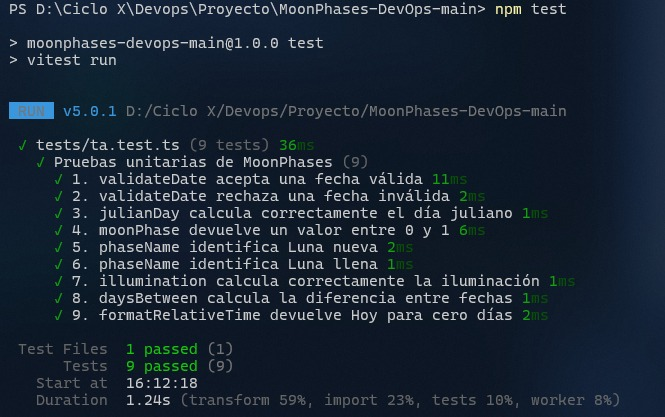
\includegraphics[width=0.80\textwidth]{content/imgs/k1.jpeg}
    \caption{Pruebas unitarias de MoonPhases.}
\end{figure}
